\documentclass[aspectratio=169]{beamer}
%
% Choose how your presentation looks.
%
% For more themes, color themes and font themes, see:
% http://deic.uab.es/~iblanes/beamer_gallery/index_by_theme.html
%
\mode<presentation>
{
    \usetheme{default}      % or try Darmstadt, Madrid, Warsaw, ...
    \usecolortheme{default} % or try albatross, beaver, crane, ...
    \usefonttheme{default}  % or try serif, structurebold, ...
    \setbeamertemplate{navigation symbols}{}
    \setbeamertemplate{caption}[numbered]
}

\usepackage[english]{babel}
\usepackage[utf8]{inputenc}
\usepackage{graphicx}
\usepackage{breqn}
\usepackage{bbm}

\newenvironment{wideitemize}{\itemize\addtolength{\itemsep}{10pt}}{\enditemize}
\newenvironment{transitionframe}{
    \setbeamercolor{background canvas}{bg=white}
    \begin{frame}}{
    \end{frame}
}

\DeclareMathOperator*{\argmax}{arg\,max}
\DeclareMathOperator*{\argmin}{arg\,min}

\usepackage[style=authoryear, backend=biber]{biblatex}
\addbibresource{econ281_presentation.bib}

\title{Flatter experience-wage profiles and declining labor force nonparticipation}
\author{Churn Ken Lee}
\institute{UC San Diego}
\date{}

\begin{document}

\frame{\titlepage}

\begin{frame}
    \frametitle{Motivation}

    Declining labor force participation among prime-aged low-skilled men (Binder \& Bound JEP 2019)
    \begin{figure}[t]
        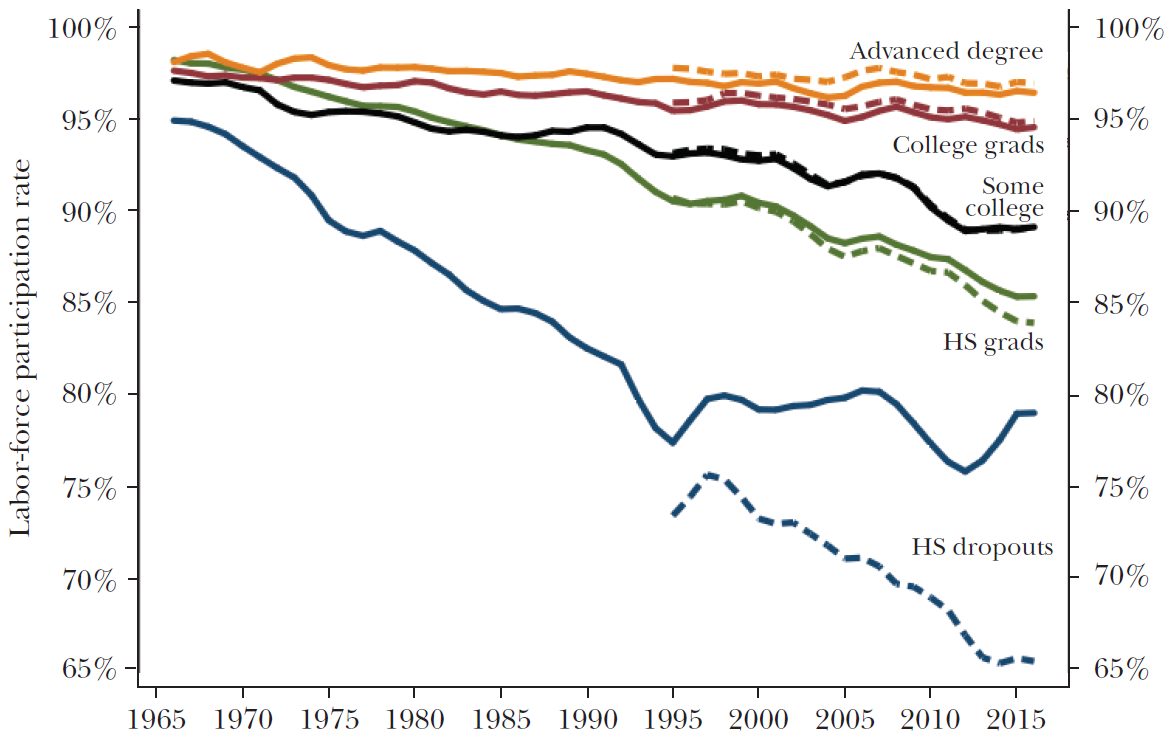
\includegraphics[width=0.7\textwidth]{../output/participation_education.png}
        \centering
    \end{figure}

\end{frame}

\begin{frame}
    \frametitle{Motivation}

    Flattening of experience-income profile of low-skilled relative to high-skilled (Elsby \& Shapiro AER 2012)
    \begin{figure}[t]
        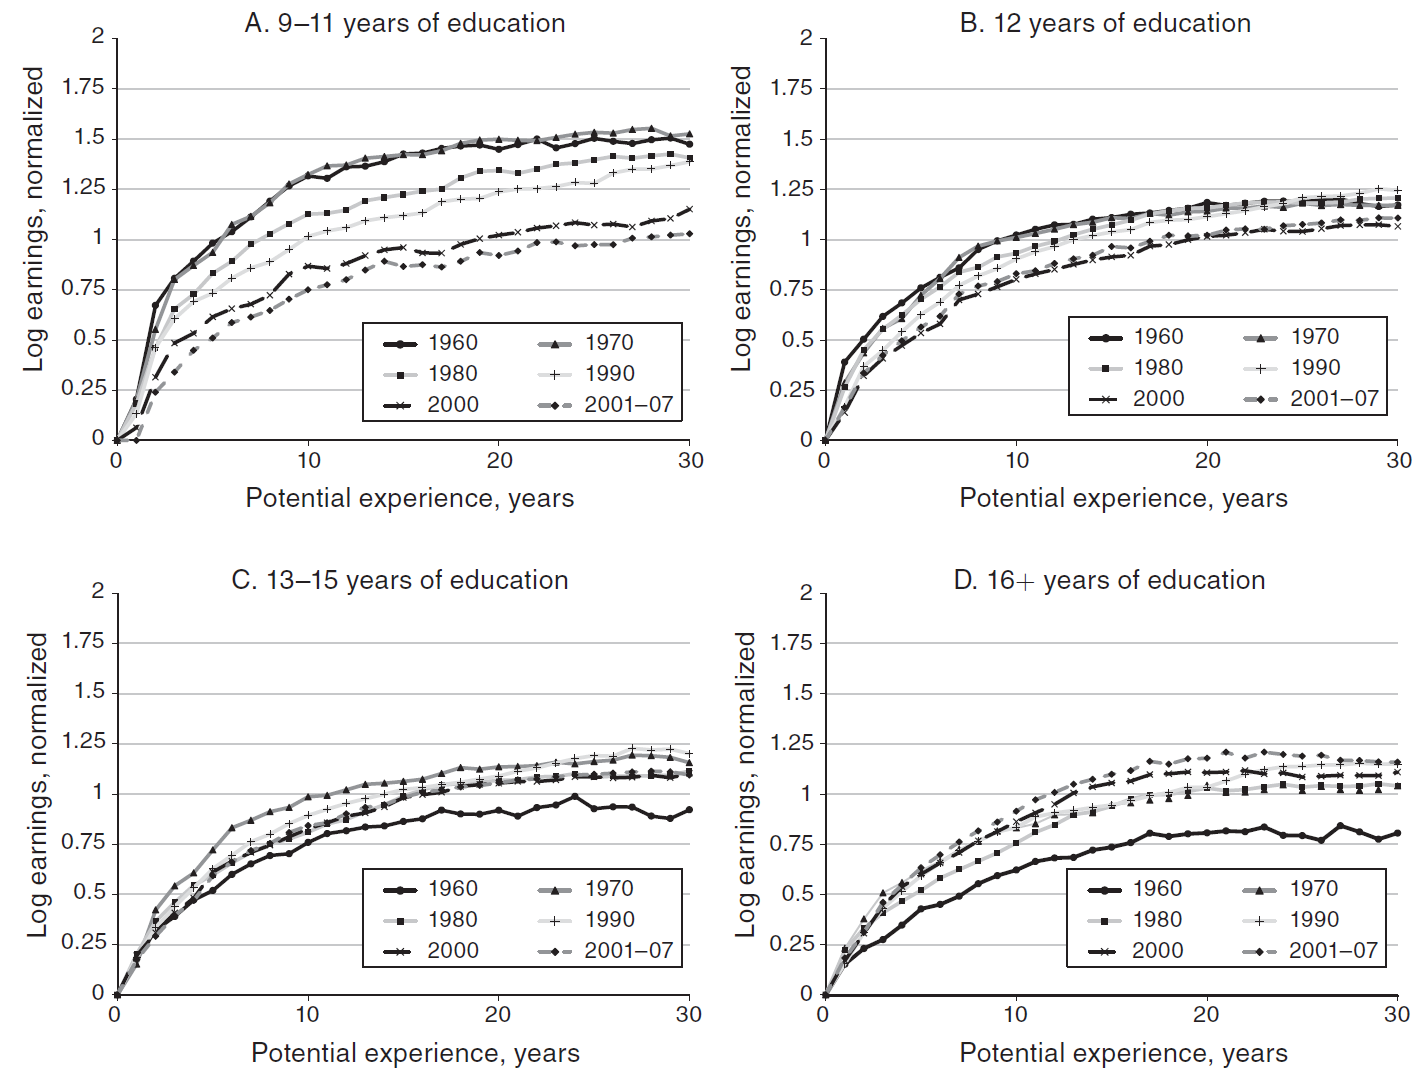
\includegraphics[width=0.65\textwidth]{../output/profile_cross_elsby_shapiro.png}
        \centering
    \end{figure}
\end{frame}

\begin{frame}
    \frametitle{Motivation}

    Flattening of experience-income profile of low-skilled relative to high-skilled (Elsby \& Shapiro AER 2012)
    \begin{figure}[t]
        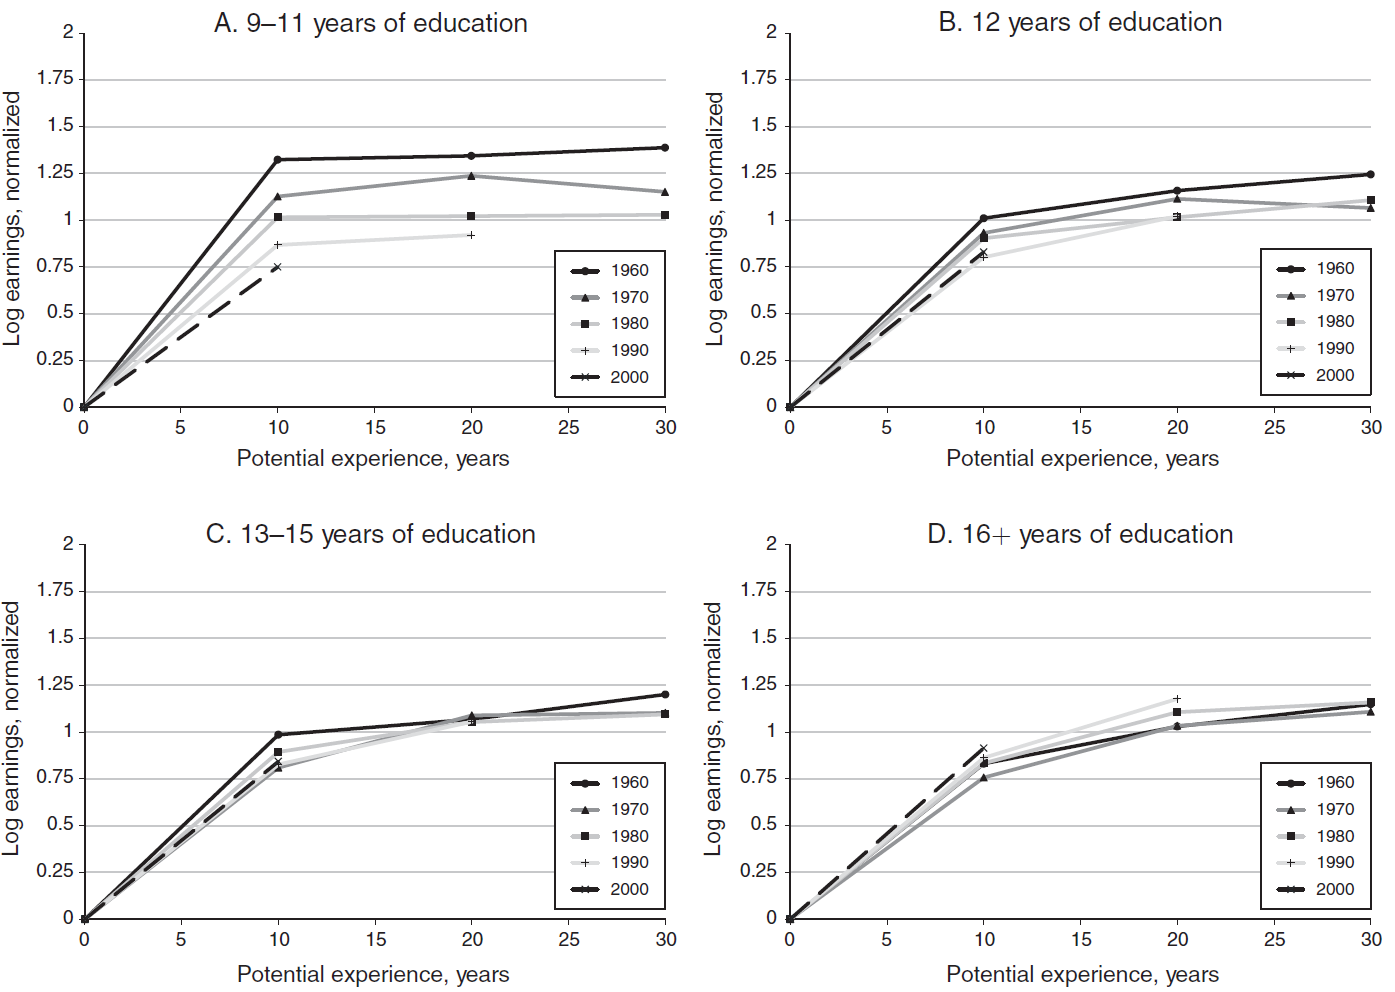
\includegraphics[width=0.65\textwidth]{../output/profile_cohort_elsby_shapiro.png}
        \centering
    \end{figure}

\end{frame}

\begin{frame}
    \frametitle{Motivation}

    Experience-income profile of lowest-skilled has actually steepened recently!
    \begin{figure}[t]
        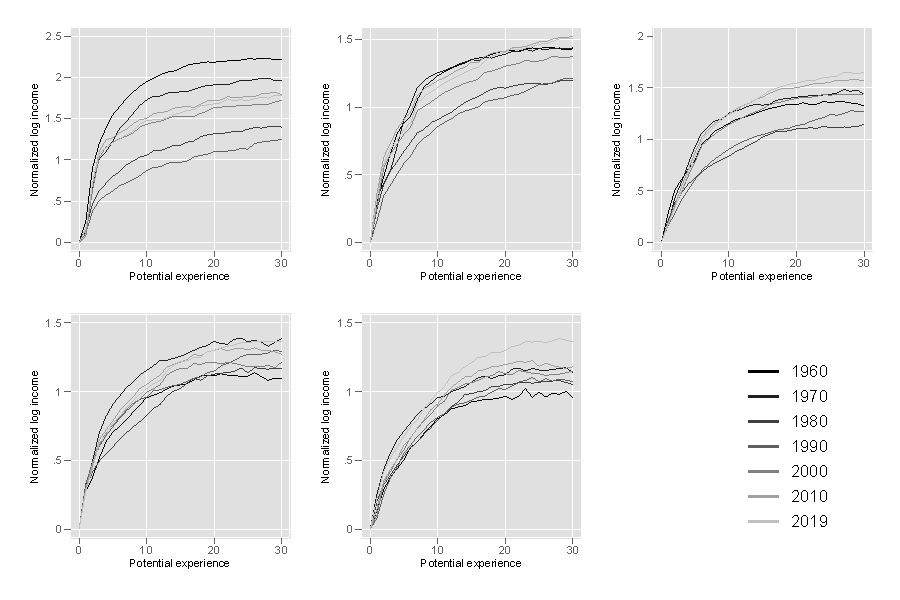
\includegraphics[width=0.8\textwidth]{../output/exp_wage_profile_cross.pdf}
        \centering
    \end{figure}
\end{frame}

\begin{frame}
    \frametitle{Motivation}

    Experience-income profile of lowest-skilled has actually steepened recently!
    \begin{figure}[t]
        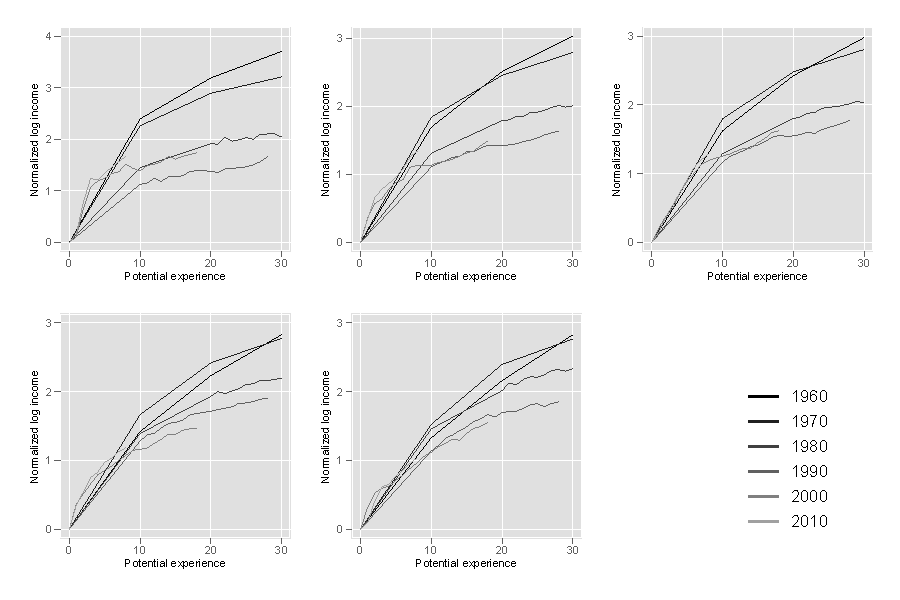
\includegraphics[width=0.8\textwidth]{../output/exp_wage_profile_cohort.pdf}
        \centering
    \end{figure}
\end{frame}

\begin{frame}
    \frametitle{Motivation}

    Increase in gap of retirement age between high and low-skilled (Rutledge 2018)
    \begin{figure}[t]
        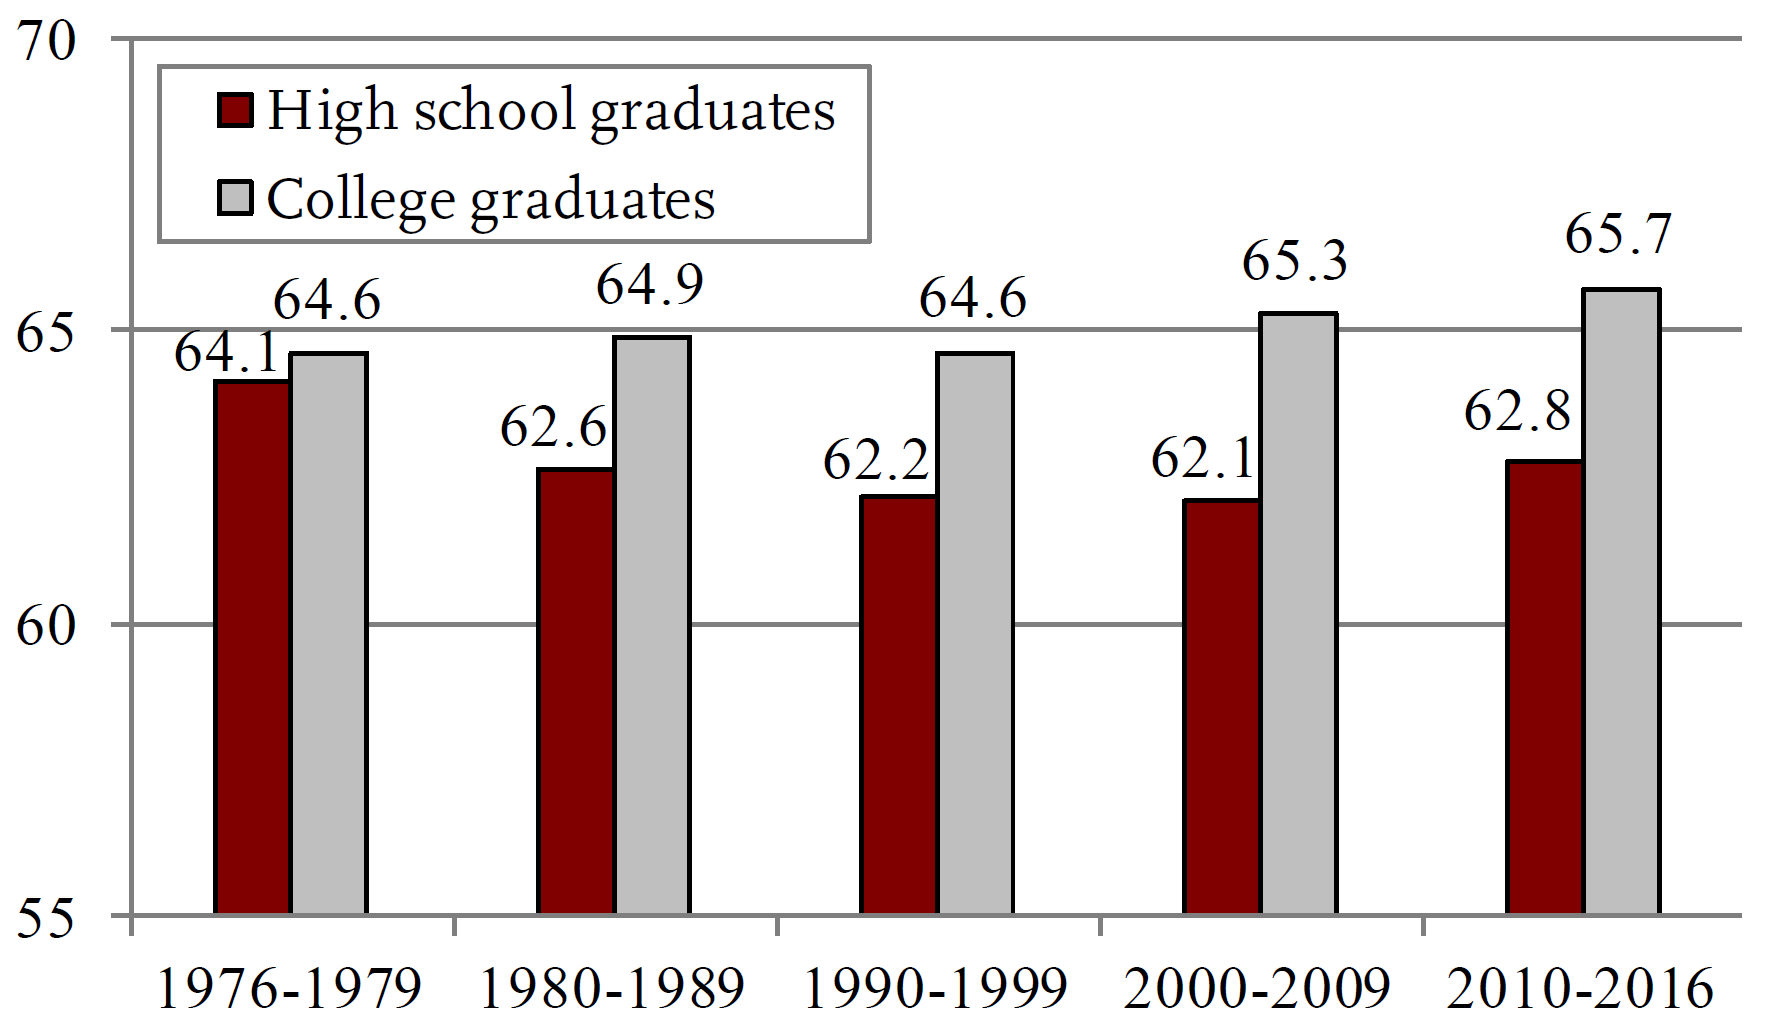
\includegraphics[width=0.8\textwidth]{../output/retirement.png}
        \centering
    \end{figure}

\end{frame}


\begin{frame}
    \frametitle{Idea}
    Declining returns to accumulation of human capital leads to
    \begin{wideitemize}
        \item less human capital accumulation
        \item lower participation
        \item and earlier retirement
    \end{wideitemize}
    among low-skilled, and lower human capital level leads to
    \begin{wideitemize}
        \item higher sensitivity and persistence to shocks
    \end{wideitemize}

\end{frame}

\begin{frame}
    \frametitle{Literature}
    Many explanations for declining LFP of prime-aged men:
    \begin{wideitemize}
        \item Skill-biased technical change (Card \& Dinardo 2002, Acemoglu \& Autor 2010)
        \item Job polarization (Foote \& Ryan 2015)
        \item Improvements in leisure technology (Aguiar et. al. 2018)
        \item Disability and SSDI (Autor \& Duggan QJE 2003, Krueger 2017)
        \item Incarceration (Binder \& Bound JEP 2019)
    \end{wideitemize}
    

\end{frame}

\begin{frame}
    \frametitle{Elements I need in my model}

    \begin{wideitemize}
        \item Human capital accumulation
        \item Education
        \item Labor supply
        \item Retirement
    \end{wideitemize}

\end{frame}

\begin{frame}
    \frametitle{Blinder-Weiss 1976}
    Agents with finite lifespan $T$ maximize lifetime utility
    \begin{equation*}
        \max_{\{ c_t \}_{t=0}^T, \{ h_t \}_{t=0}^T, \{ x_t \}_{t=0}^T} \sum_{t=0}^{T} \beta^t u(c_t, 1-h_t) + B(A_{T+1})
    \end{equation*}
    subject to
    \begin{equation*}
        A_{t+1} = (1+r)A_{t} + h_t g(x_t)K_{t} - c_{t},
    \end{equation*}
    \begin{equation*}
        K_{t+1} = (1-\delta)K_t + x_t h_t K_t,
    \end{equation*}
    \begin{equation*}
        x_t ,h_t \in [0,1],
    \end{equation*}
    \begin{wideitemize}
        \item $x_t$ and $g(x_t)$ governs tradeoff between accumulating human capital and earnings
        \item $B$ is bequest, $A$ is assets, and $K$ is human capital
    \end{wideitemize}

\end{frame}

\begin{frame}
    \frametitle{$g(x)$}
    
    \begin{figure}[t]
        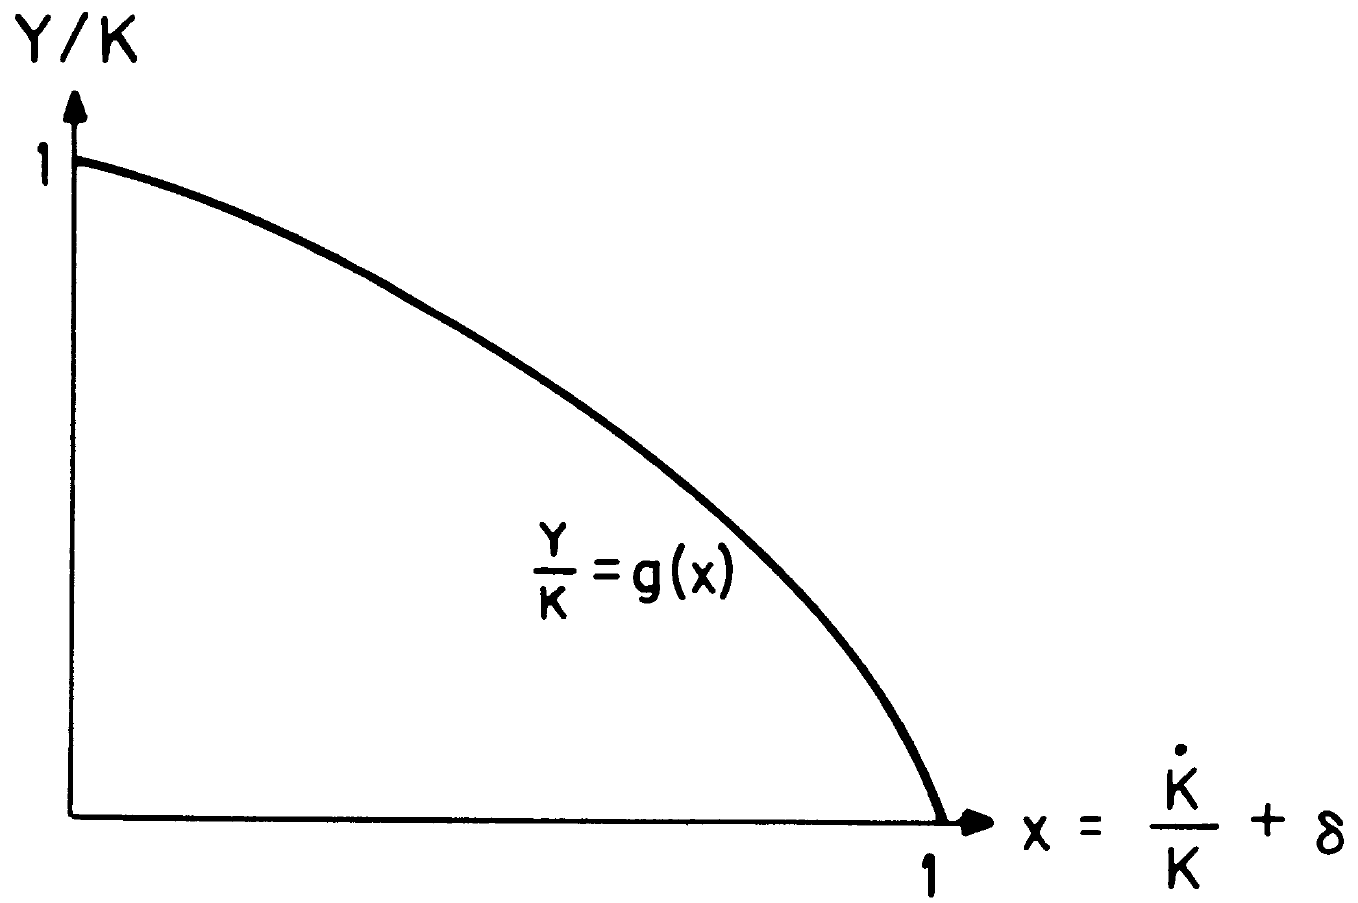
\includegraphics[width=0.8\textwidth]{../output/g.png}
        \centering
    \end{figure}

\end{frame}



\begin{frame}
    \frametitle{Endogenous life phases}
    
    Four phases:
    \begin{wideitemize}
        \item Education: $x = 1$
        \item Work + learning: $0 < x < 1$
        \item Work + no learning: $x = 0$
        \item Retirement: $h = 0$
    \end{wideitemize}

\end{frame}

\begin{frame}
    \frametitle{Endogenous life phases}

    \begin{figure}[t]
        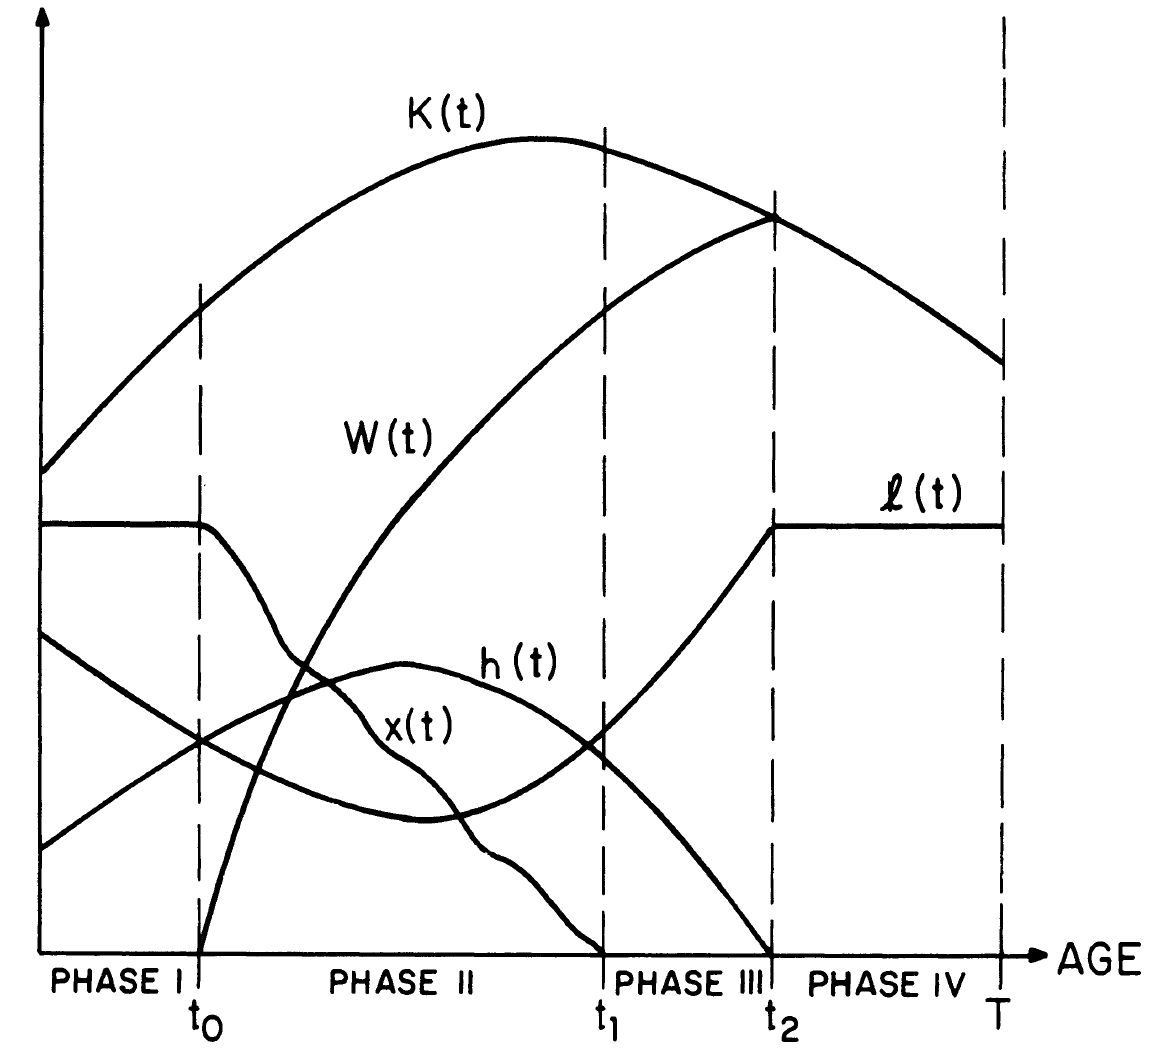
\includegraphics[width=0.6\textwidth]{../output/phases.png}
        \centering
    \end{figure}

\end{frame}



\begin{frame}
    \frametitle{Challenges}

    \begin{wideitemize}
        \item Both shooting method (continuous time model) and backward induction of value function (discrete time model) not working
        \item Possible way forward: discretize labor supply and investment decisions (Keane \& Wolpin 1994)
        \item What is $g(x)$?
        \item What is causing the flattening and steepening of the experience-income profile?
        \begin{wideitemize}
            \item Changes in labor markets; incorporate into the $g(x)$ function?
            \item Changes in monopsony power?
            \item Endogenize changes in the slope of experience-income profile
        \end{wideitemize}
    \end{wideitemize}

\end{frame}

\begin{frame}
    \frametitle{HJB}

    The HJB equation for the agent's problem is
    \begin{align*}
        \rho V(A, K, t) = \max_{c, h, x} \quad &u(c, 1-h) \\
        &+ \partial_A V(A, K, t) \left[rA + h g(x) K - c \right] \\
        &+ \partial_K V(A, K, t) \left[-\delta K + x h K \right] \\
        &+ \partial_t V(A, K, t)
    \end{align*}

\end{frame}

\begin{frame}
    \frametitle{Finite difference approximation of the HJB}

    \begin{wideitemize}
        \item $nA$ and $nK$ are the number of grid points for $A$ and $K$
        \item Denote the index for $A$ and $K$ as $i$ and $j$ respectively
        \item Denote $V(A_i, K_j, t) = V_{ij}^t$
        \item Denote drift in $A$ as $\mu_A$, drift in $K$ as $\mu_K$
    \end{wideitemize}

\end{frame}

\begin{frame}
    \frametitle{Forward and backward difference approximation}

    \begin{wideitemize}
        \item Forward difference:
        \begin{align*}
            \partial_A^F V_{i,j}^t &= \frac{V_{i+1, j}^t - V_{i, j}^t}{\Delta A} \\
            \partial_K^F V_{i,j}^t &= \frac{V_{i, j+1}^t - V_{i, j}^t}{\Delta K}
        \end{align*}
        \item Backward difference:
        \begin{align*}
            \partial_A^B V_{i,j}^t &= \frac{V_{i, j}^t - V_{i-1, j}^t}{\Delta A} \\
            \partial_K^B V_{i,j}^t &= \frac{V_{i, j}^t - V_{i, j-1}^t}{\Delta K}
        \end{align*}
    \end{wideitemize}

\end{frame}

\begin{frame}
    \frametitle{Choice of forward or backward difference}

    \begin{wideitemize}
        \item At any grid point $i, j$ at time $t$, solve for $c, h, x$:
        \begin{align}
            \partial_c u(c_{i,j}^t, h_{i,j}^t) &= \partial_A V_{i,j}^t
        \end{align}
        \begin{align}
            \partial_h u(c_{i,j}^t, h_{i,j}^t) &= \partial_A V_{i,j}^t \left[ g(x_{i, j}^t) K_{j} \right] + \partial_K V_{i,j}^t \left[ x_{i, j}^t K_{j} \right] \quad \text{if} \quad 0 < h < 1 \\
            \partial_h u(c_{i,j}^t, h_{i,j}^t) &\geq \partial_A V_{i,j}^t \left[ g(x_{i, j}^t) K_{j} \right] + \partial_K V_{i,j}^t \left[ x_{i, j}^t K_{j} \right] \quad \text{if} \quad h = 0
        \end{align}
        \begin{align}
            \partial_K V_{i,j}^t \left[ h K_{j} \right] &= -\partial_A V_{i,j}^t \left[ h g'(x_{i, j}^t) K_{j} \right] \quad \text{if} \quad 0 < x < 1  \\
            \partial_K V_{i,j}^t \left[ h K_{j} \right] &\geq -\partial_A V_{i,j}^t \left[ h g'(x_{i, j}^t) K_{j} \right] \quad \text{if} \quad x = 1  \\
            \partial_K V_{i,j}^t \left[ h K_{j} \right] &\leq -\partial_A V_{i,j}^t \left[ h g'(x_{i, j}^t) K_{j} \right] \quad \text{if} \quad x = 0
        \end{align}
        \item Problem: Do we use $\partial_A^F$ or $\partial_A^B$, and $\partial_K^F$ or $\partial_K^B$?
    \end{wideitemize}

\end{frame}

\begin{frame}
    \frametitle{Choice of forward or backward difference}

    \begin{wideitemize}
        \item Backwards in $A$, forwards in $K$: $\partial_A^B + \partial_K^F \Rightarrow \mu_A^{BF}, \mu_K^{BF}$
        \item Choose approximation scheme that is consistent with computed drift
        \item e.g., $\partial_A^B + \partial_K^F$ requires $\mu_A^{BF} < 0, \mu_K^{BF} > 0$
        \item Consistent scheme may not always exist:
        \begin{wideitemize}
            \item Boundaries
            \item Steady-states
        \end{wideitemize}
        \item May have more than 1 consistent scheme due to non-concavity of $V$
    \end{wideitemize}

\end{frame}

\begin{frame}
    \frametitle{Discretizing HJB}
    \begin{wideitemize}
        \item Stack all $V_{i, j}^{t+1}$ into $V^{t+1}$, a vector of length $nA * nK$
        \item $V^{t+1}$ has associated optimal $c^t, h^t, x^t$, flow utility $U(V^{t+1})$, and drifts $\mu^t$
        \item At each $i, j$, there is an associated upwind direction for $\partial V$
        \item Matrix $A(V^{t+1})$ encodes these directions and drifts $\mu^{t+1}$, so $A(V^{t+1})*V^{t+1} = \partial V^{t+1}*\mu^{t+1}$
    \end{wideitemize}
    
\end{frame}

\begin{frame}
    \frametitle{Discretizing HJB}
    Recall HJB:
    \begin{align*}
        \rho V(A, K, t) = \max_{c, h, x} \quad &u(c, 1-h) \\
        &+ \partial_A V(A, K, t) \left[rA + h g(x) K - c \right] \\
        &+ \partial_K V(A, K, t) \left[-\delta K + x h K \right] \\
        &+ \partial_t V(A, K, t)
    \end{align*}
    Discretized and stacked version:
    \begin{equation}
        \rho V^{t} = U(V^{t+1}) + A(V^{t+1}) * V^{t} + \frac{V^{t+1} - V^{t}}{\Delta t}
    \end{equation}
    \begin{wideitemize}
        \item Solve backwards from terminal bequest motive: $V^T = B(A^T)$
    \end{wideitemize}
    
\end{frame}

\begin{frame}
    \frametitle{Boundaries}

    \begin{wideitemize}
        \item What do we do at $A_{min}$, $A_{max}$, $K_{min}$, and $K_{max}$?
        \item Problem: need $\mu_{A} \geq 0$ at $A_{min}$ and $\mu_{A} \leq 0$ at $A_{max}$
        \item Possible solution: make $A_{max}$ very large so that $\mu_{A}^{BF}, \mu_{A}^{BB} < 0$ naturally at $A_{max}$
        \item Choose $BF$ or $BB$ according to consistency with $\mu_{K}$
        \item Cannot make $A_{min}$ very small, e.g., borrowing constraint $\bar{A} = A_{min}$
        \item If $\mu_A^{FF}, \mu_A^{FB} < 0$ at $A_{min}$, then set $\partial_A$ at $A_{min}$ so that $\mu_A^{FF}, \mu_A^{FB} = 0$
        \item Note: possible to have steady-state in $K$ when at $A$ boundary, and vice versa
    \end{wideitemize}

\end{frame}

\begin{frame}
    \frametitle{Steady-state in one dimension}

    \begin{wideitemize}
        \item What do we do when one of the state variables is never consistent?
        \item e.g., $\mu_A^{FF}, \mu_A^{FB} > 0$, so $A$ is consistent in the $F$ direction
        \item but $\mu_K^{FF} < 0$ and $\mu_K^{FB} > 0$
        \item I set $K$ to be at steady-state
        \item Do so by setting $\partial_K$ so that $\mu_K = 0$
        \item We will get $\partial_A^F, \partial_K \Rightarrow \mu_A > 0, \mu_K = 0$
    \end{wideitemize}

\end{frame}

\begin{frame}
    \frametitle{Steady-state in both dimensions}

    \begin{wideitemize}
        \item Steady-state in both dimension, so both $A$ and $K$ are inconsistent
        \item We don't have a consistent $\mu_A^{FF}, \mu_A^{FB} > 0$, or $\mu_A^{BF}, \mu_A^{BB} < 0$
        \item Neither do we have a consistent $\mu_K^{FF}, \mu_K^{BF} > 0$, or $\mu_K^{FB}, \mu_K^{BB} < 0$
        \item Then set $\partial_A$ and $\partial_K$ such that $\mu_A = 0$ and $\mu_K = 0$
    \end{wideitemize}

\end{frame}


\begin{frame}
    \frametitle{Non-concavity of $V$}

    \begin{wideitemize}
        \item With concave $V$, $\partial_A^F < \partial_A^B$
        \item $\Rightarrow \mu_A^{FF} < \mu_A^{BF}$
        \item We will not have $A$ consistent in both $F$ and $B$:
        \begin{wideitemize}
            \item $\mu_A^{BF} < 0 <\mu_A^{FF}$ contradicts $\mu_A^{FF} < \mu_A^{BF}$
        \end{wideitemize}
        \item However, this may happen with non-concave $V$
        \item Solution: choose approximation that leads to larger Hamiltonian value
    \end{wideitemize}

\end{frame}


\begin{frame}
    \frametitle{Progress since last meeting}
    
    \begin{wideitemize}
        \item Improved algorithm explanation slides
        \item Met with Johannes:
        \begin{wideitemize}
            \item He suggested I fix terminal condition spike by increasing bequest motive (completed, seems to work, not sure if best solution, will try others)
            \item He thinks my modified algorithm to impose boundary/steady state/boundary + steady state conditions seem reasonable
            \item He suggested a modification for rare cases where boundary/steady state coincide with non-concavity ambiguity: add tie-breaking (will need to wrap boundary/steady state condition checkers inside functions; 40\% done)
            \item Create 1-slide explainer (what does Titan think?)
        \end{wideitemize}
        \item Not completed: Look at data and calibrate (will do after algorithm is faster)
    \end{wideitemize}

\end{frame}

\begin{frame}
    \frametitle{One-slide explainer}

    \begin{wideitemize}
        \item Discretize HJB over grids of $A, K$ indexed by $i, j$:
        \item Approximate derivatives of $V$ using finite difference
        \item Forward difference: 
        \begin{equation}
            \partial_A V(A_i, K_j, t) = \frac{V(A_{i+1}, K_j, t) - V(A_{i}, K_j, t)}{\Delta A}
        \end{equation}
        \item Backward difference: 
        \begin{equation}
            \partial_A V(A_i, K_j, t) = \frac{V(A_{i}, K_j, t) - V(A_{i-1}, K_j, t)}{\Delta A}
        \end{equation}
        \item Choose direction and optimal choice via ``upwind scheme'': direction is consistent with drift of state variable implied by optimal choice
        \item Once we know $V^{t+1}$, only unknown in discretized HJB is $V^t$
        \item Solve backwards from terminal $V^T$
    \end{wideitemize}

\end{frame}

\begin{frame}
    \frametitle{Current computational issues}

    \begin{wideitemize}
        \item Proving my algorithm satisfies the three conditions of Barles and Souganidis (1991) (monotonicity, consistency, stability)
        \item Speed up computation by consolidating ambiguous case checkers within a single function (goes hand-in-hand with Johannes' suggestion)
        \item Length of time in schooling depends on initial wealth due to credit constraint
        \begin{wideitemize}
            \item With too much assets, agents end up not accumulating much human capital or assets
            \item With too little assets, $x = 1$ period is very short
            \item May need to allow for debt? Will require modified bequest motive
        \end{wideitemize}
    \end{wideitemize}

\end{frame}

\begin{frame}
    \frametitle{Path of choice variables}
    
        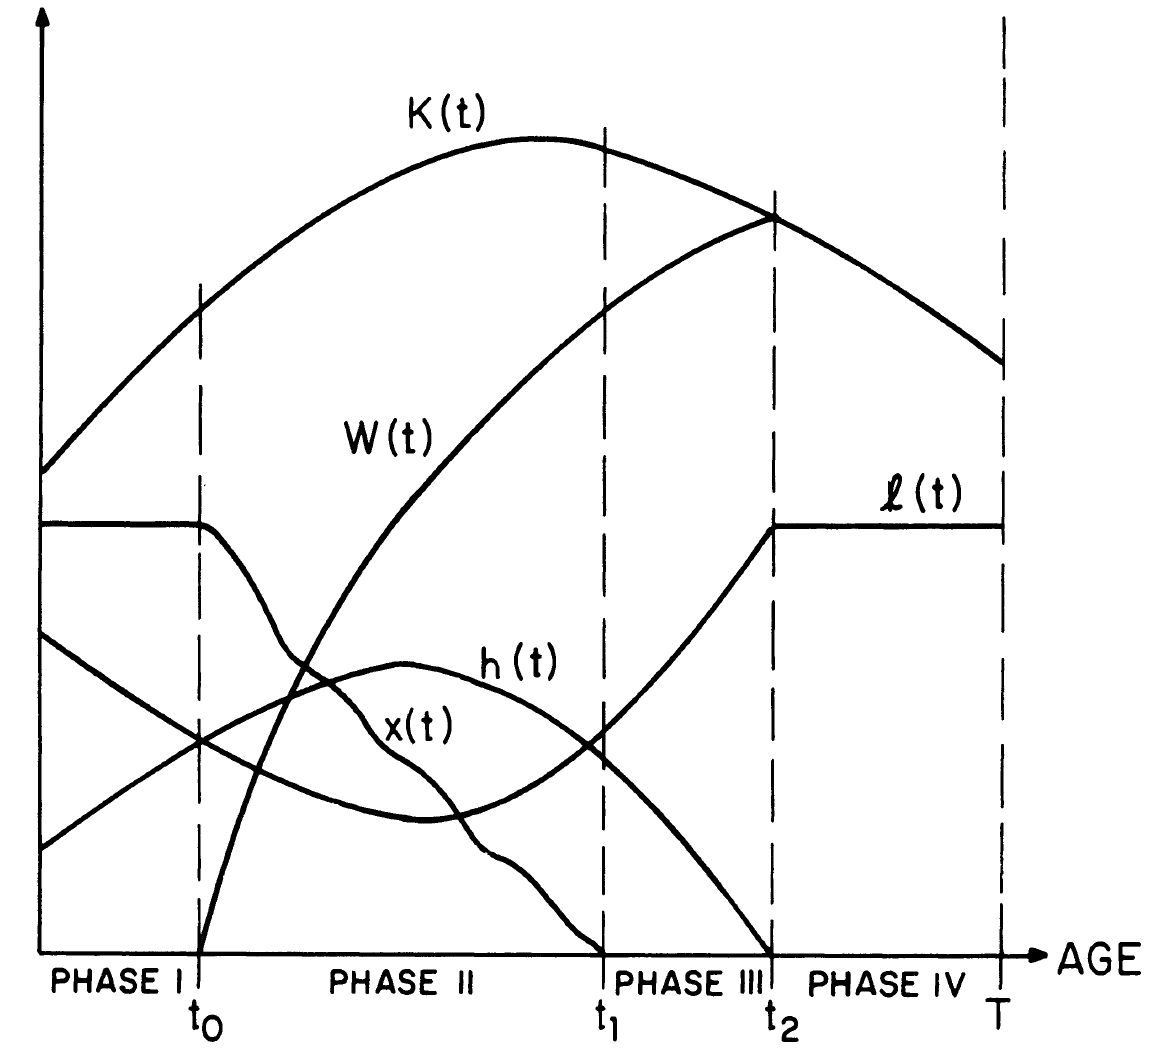
\includegraphics[width=0.49\textwidth]{../output/phases.png}
        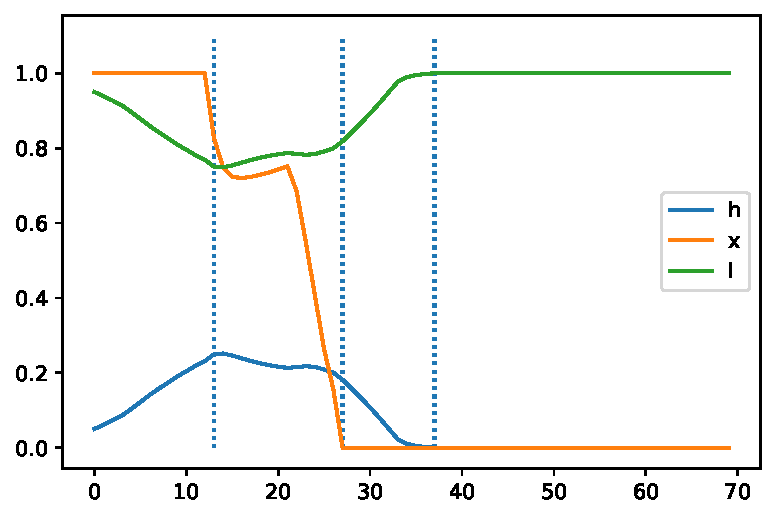
\includegraphics[width=0.49\textwidth]{../output/fd_hjb_choice_path.pdf}

\end{frame}

\begin{frame}
    \frametitle{Path of state variables}
    
        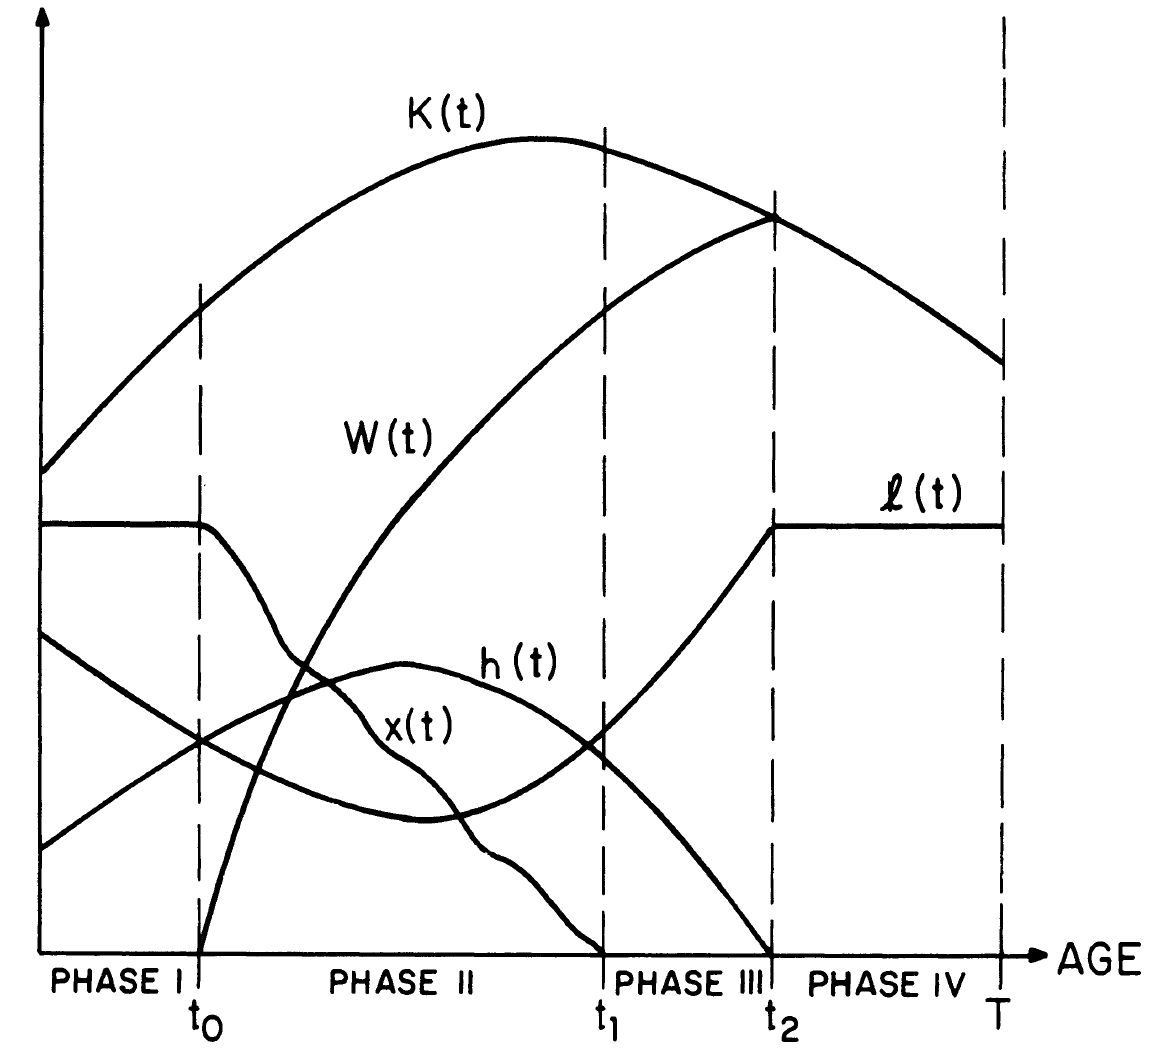
\includegraphics[width=0.49\textwidth]{../output/phases.png}
        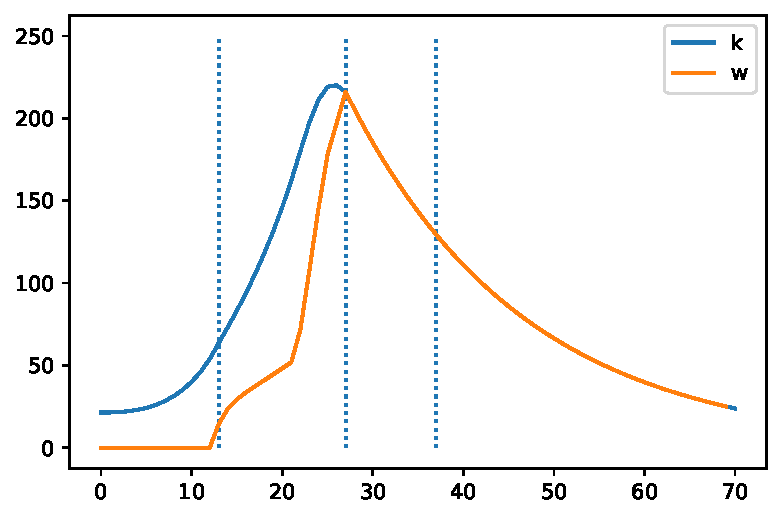
\includegraphics[width=0.49\textwidth]{../output/fd_hjb_state_path.pdf}

\end{frame}

\end{document}
